%
% ****
\chapter{Kinematisches Model}
% ****
%
Im folgenden Kapitel wird das kinematische Model des \kuka \ anhand der geometrischen sowie mechanischen Struktur hergeleitet. Der Roboter kann als offene kinematische Kette aus Starrkörpern, welche durch Schub- oder Drehgelenke miteinander verbunden sind \cite{Siciliano:2008:RMP:1524151}. Zur Beschreibung des Endeffektors in kartesischen Koordinaten wird eine Transformation vom Arbeitsraum in den Gelenksraum benötigt.  Zur einheitlichen Definition der kartesischen Achsen $x,y,z$ wird die Denavit-Hardenberg-Konvention verwendet. 

\section{Arbeits- , Konfigurations- und Gelenksraum}
Ein anthropomorpher Roboter spannt einen kugelförmigen, dreidimensionalen Arbeitsraum $\mathcal{A} = \R^3 $, welcher durch das Basis-Koordinatensystem $[x_b,y_b,z_b]^T$ beschrieben wird, auf. Der Konfigurationsraum enthält im Gegenteil zum Arbeitsraum nicht nur die erreichbare Position $p_b^e = [x_b^e, y_b^e, z_b^e]^T$ des Endeffektors im Basis-Koordinatensystem, sondern auch die Orientierung $\phi_b^e = [\varphi_b^e, \vartheta_b^e, \psi_b^e]^T$. Folglich führt die Darstellung im Konfigurationsraum zu 
\begin{align}
x_b^e = 
\begin{bmatrix}
p_b^e \\
\phi_b^e
\end{bmatrix}.
\end{align}
Die Darstellung der Rotation vom Endeffektor- in das Basis-Koordinatensystem mittels der Euler-Winkel $\varphi_b^e, \theta_b^e$ und $\psi_b^e$ ist die minimale Form der Orientierungsdarstellung. Durch diese Darstellung können Singularitäten dadurch entstehen, dass zwei der drei Drehachsen parallel zueinander liegen, wodurch das System einen Freiheitsgrad weniger besitzt. Dies wird vermieden, indem die Darstellung durch Einheits-Quaternionen hinzugezogen wird. Die Euler-Winkel 
\begin{align}
\phi_b^e &= \arctan \left( \frac{R_{2,3}}{R_{1,3}} \right) \\
\vartheta_b^e &= \arctan \left( \frac{\sqrt{R_{2,3}^2 + R_{1,3}^2} }{R_{3,3}}\right) \\
\psi_b^e &= \arctan \left( \frac{R_{3,2}}{-R_{3,1}} \right)
\end{align}
können aus der Rotationsmatrix ausgerechnet werden. \\

Der Gelenksraum $\mathcal{G} = \R^n$ wird durch die $n$ Gelenke aufgespannt. Für den \kuka \ beträgt $n = 7$ , wobei der Vektor $\vec{q} = [q_1,...,q_n]^T$ die Winkel jedes der sieben Dreh-Gelenke enthält, welcher die Rotation um die $z_i$-Achse  des jeweiligen Gelenks-Koordinatensystem $0_i$, mit $i \in {1,...,n}$ beschreibt. Dies wird Gelenkskonfiguration bezeichnet. Der erreichbare Gelenksraum $\mathcal{G}^e$ stellt dabei eine Einschränkung von $\mathcal{G}$ durch die eingeschränkte Rotation der Gelenke. Daraus folgt 
\begin{align}
\mathcal{G}^e = \{ \vec{q} \in \mathcal{G} \ | \ q_{i,min} < q_i < q_{i,max}, \ \ \ \forall i \in 1,...,n \}.
\end{align}
Die direkte Kinematik $ \vec{k} : \mathcal{G}^e \rightarrow \mathcal{A}$ bildet den Gelenksraum auf den euklidischen Raum ab. Die kartesischen Koordinaten können somit durch 
\begin{align}
\vec{x} = \vec{k}(\vec{q})
\end{align}
berechnet werden. 


\section{Denavit-Hartenberg Transformation}
Für die Denavit-Hartenberg Transformation, im Folgenden DH-Parameter,  wird zwischen den klassischen und den modifizierten DH-Parametern differenziert. Diese unterscheiden sich in der Reihenfolge der translatorischen und rotatorischen Bewegung bezüglich der $x$ und $z$-Achse. Für die klassischen DH-Parameter wird zuerst die Rotation und Translation um die $z_{i-1}$-Achse und danach die Translation und Rotation um die $x_i$-Achse. Im Folgenden werden die klassischen DH-Parameter berücksichtigt. \\

\begin{table}[htb]
\centering
	\begin{tabular}{lcccc}\toprule
		i &$a_i$ \ \ \  	&$\alpha_i$ \ &$d_i$ \ &$\theta_i$	\\
		\midrule
	   $1$	&$0$		 &-$\pi/2$	& $d_{bs}$  	&$\theta_1$  \\
	   $2$	&$0$		 &$\pi/2$	& $0 $	        &$\theta_2$  \\
	   $3$	&$0$		 &$\pi/2$	& $d_{se}$  	&$\theta_3$  \\
	   $4$	&$0$		 &-$\pi/2$	& $0$	        &$\theta_4$  \\
	   $5$	&$0$		 &-$\pi/2$	& $d_{ew}$    	&$\theta_5$  \\
	   $6$	&$0$		 &$\pi/2$	& $0$	        &$\theta_6$  \\
	   $7$	&$0$		 &$0$	        & $d_{wf}$   	&$\theta_7$  \\ \bottomrule

	\end{tabular}
	\caption{Klassische Denavit-Hardenberg Parameter für den \kuka, wobei $d_{bs}$ die Distanz zwischen der Basis und Schulter, $d_{se}$ zwischen Schulter und Ellenbogen, $d_{ew}$ zwischen Ellenbogen und Handgelenk und $d_{wf}$ zwischen Handgelenk und Werkzeug ist.}
		\label{tab:DH_Parameter}
	\end{table}
 Die DH-Parameter des \kuka \ sind in Tabelle \ref{tab:DH_Parameter} dargestellt. Die translatorischen Verschiebung in $x_i$-Richtung ist für alle Gelenke gleich null, da die Links nur mittels Drehgelenken miteinander verbunden sind. Die homogene Transformation 
\begin{align}
H_0^e = 
\begin{bmatrix}
R_0^e & d_0^e \\
0^T & 1 \\
\end{bmatrix}, \qquad  R_0^e \in SO(3)
\end{align}
beschreibt die Transformation vom Endeffektor- ins Basis-Koordinatensystem, wobei $R_0^e$ die Rotation und $d_0^e$ die Translation darstellen.
\begin{figure}[h]
	\centering
	\begin{tikzpicture}
\draw [ thick,->,>={Straight Barb[]}] (0,0) -- (0,6);
\draw [ thick,->,>={Straight Barb[]}] (0,0) -- (8,0);
\large{
\node at (7.8,-.5) {$x_0$};
\node at (-.5,5.8) {$y_0$};
\node at (-.3,-.3) {$0_0$};
}

\draw [blue, thick,dashed] (3.5,3)-- (5.4,3);
\draw [blue, thick,->,>={Straight Barb[]}] (3.5,3) -- (5.6,4.1);
\draw [blue, thick,->,>={Straight Barb[]}] (3.5,3) -- (2.5,4.8);
\draw [blue, thick,->,>={Straight Barb[]}] (3.5,3) -- (4,4.5);
\draw [thick,->,>={Straight Barb[]}] (0,0) -- (3.5,3);
\draw [thick,->,>={Straight Barb[]}] (0,0) -- (3.5,3);
\draw [thick,->,>={Straight Barb[]}] (0,0) -- (4,4.5);

\draw [blue, thick,->,>={Straight Barb[]}] (4.9,3) to [out=90,in=297.65] (4.74,3.65);
\large{
\node at(4,4.8) {$P$};
\node at (5.7,3.7) {\textcolor{blue}{$x_1$}};
\node at (2.2,4.6) {\textcolor{blue}{$y_1$}};
\node at (3.8,2.7) {\textcolor{blue}{$0_1$}};
\node at (4.2,4.1) {\textcolor{blue}{$\vec{p}_1$}};
\node at (1.8,2.5) {$\vec{p}_0$};
\node at (4.4,3.2) {\textcolor{blue}{$\theta$}};
\node at (2.5,1.7) {$\vec{d}_0^1$};
}
\end{tikzpicture}
	\caption{Die Bildunterschrift sollte eine sinnvolle Erläuterung der
		Darstellung geben und ist immer mit einem Satzpunkt abzuschließen.}
	\label{fig:Koordinaten_trans}
\end{figure}
Mit der Rotationsmatrizen $Rot_{zi}$ und $Rot_{xi}$ um die $z_{i-1}$-  und $x_{i}$-Achse, der translatorische Verschiebungen $Trans_{zi}$ und $Trans_{xi}$

\begin{align}
Rot_{zi} &= 
\begin{bmatrix}
	\cos\theta_i & -\sin\theta_i & 0 & 0 \\
	\sin\theta_i & \cos\theta_i  & 0 & 0 \\
	0            & 0             & 1 & 0 \\
	0            & 0             & 0 & 1 
\end{bmatrix}
, 
\qquad \, \, Trans_{zi} = 
\begin{bmatrix}
	1            & 0             & 0 & 0 \\
	0            & 1             & 0 & 0 \\
	0            & 0             & 1 & d_i \\
	0            & 0             & 0 & 1 
\end{bmatrix}, \\
Rot_{xi} &= 
\begin{bmatrix}
1             & 0             & 0 & 0 \\
\cos\alpha_i  & -\sin\alpha_i & 0 & 0 \\
\sin\alpha_i  & \cos\alpha_i  & 1 & 0 \\
0             & 0             & 0 & 1 
\end{bmatrix},
\qquad Trans_{xi} = 
\begin{bmatrix}
1            & 0             & 0 & a_i \\
0            & 1             & 0 & 0 \\
0            & 0             & 1 & 0 \\
0            & 0             & 0 & 1 
\end{bmatrix} 
\end{align}
kann die Transformation vom $i$-ten in das $i-1$-te Koordinatensystem folgendermaßen 

\begin{align}
H_i^{i-1} &= Rot_{zi}\ Trans_{zi}\ Trans_{xi} \ Rot{xi}\\
			  &= \begin{bmatrix}
			  \cos\theta_i  & -\sin\theta_i \cos\alpha_i     & \sin \theta_i \sin \alpha_i & a_i \cos \theta_i \\
			  \sin\theta_i  & -\sin\alpha_i                  & -\cos \theta_i \sin \alpha_i & a_i \sin \theta_i \\
			  0             & \sin\alpha_i                   & \cos \alpha_i & d_i \\
			  0             & 0                              & 0 & 1 
			  \end{bmatrix}
\end{align}
dargestellt werden. Für den \kuka \ mit sieben Gelenken gilt die Abbildung
\begin{align}
H_0^7 = H_0^1 H_1^2 H_2^3 H_3^4 H_4^5 H_5^6 H_6^7.
\end{align}
Zur Bestimmung der Transformation 
\begin{align}
H_b^e = H_b^0 H_0^7 H_7^e 
\end{align}
ist die Vereinfachung 
\begin{align}
H_b^0 = \begin{bmatrix}
1            & 0             & 0 & 0 \\
0            & 1             & 0 & 0 \\
0            & 0             & 1 & 0 \\
0            & 0             & 0 & 1 
\end{bmatrix} , \qquad 
H_7^e = \begin{bmatrix}
1            & 0             & 0 & 0 \\
0            & 1             & 0 & 0 \\
0            & 0             & 1 & d_{end} \\
0            & 0             & 0 & 1 
\end{bmatrix}
\end{align}
zu wählen, da das Basis-Koordinatensystem im $0$-ten Koordinatensystem liegt und der Endeffektor in der $z_7$-Achse liegt. 
\section{Inverse Kinematik}
Die inverse Kinematik beschreibt die Abbildung des Arbeitsraum auf den erreichbaren Gelenksraum $ \vec{k}^{-1}:\mathcal{A} \rightarrow \mathcal{G}$. Die Gelenkskoordinaten können durch 
\begin{align}
\vec{q}=\vec{k}^{-1}(\vec{x})
\end{align}
ermittelt werden. Die Lösung der inversen Kinematik $\vec{k}^{-1}$ ist nicht für alle Fälle eindeutig, da der \kuka \ sieben Freiheitsgrade besitzt, jedoch für die Position $x_b^e$ nur sechs Freiheitsgrade benötigt werden.  

\subsection{Globale Konfiguration und Armwinkel}
Zur eindeutigen Bestimmung der inversen Kinematik muss die globale Konfiguration $GK$ sowie der redundante Armwinkel $gamma$ definiert werden. Die globale Konfiguration $GK$ besteht aus drei Variablen, welche die Position der Schulter ($GK_2$ ) , des Ellenbogen ($GK_4$) sowie des Handgelenks ($GK_6$) definiert. Daraus folgt
\begin{align}
GK_i = \begin{cases}
1, \qquad &\text{für} \: \theta_i > 0\\
-1, \qquad &\text{für} \: \theta_i < 0
\end{cases}  \; ,\forall i \in {2,4,6}
\end{align}
was dem menschlichen Arm nachempfundenen Positionen Schulter links/rechts, Ellenbogen oben/unten und Handgelenk innen/außen entspricht. Der redundante Armwinkel $\gamma$ wird, wie in Abbildung \ref{fig:Elbow_redundancy} durch die $SE^vW$-Ebene, definiert. Die Position des virtuellen Ellenbogens wird durch $\theta_3^v=0$ erreicht, wodurch eine eindeutige Darstellung des Armwinkels $\gamma$ ohne Singularitäten entsteht \cite{Zhou}. Zur Bestimmung von $\gamma$ wird die globale Konfiguration vorrausgesetzt, da die Konfiguration des Ellenbogens zwischen realen und virtuellen Manipulators unterscheiden können. \\

\begin{figure}[h]
	\centering
	\scalebox{0.4}{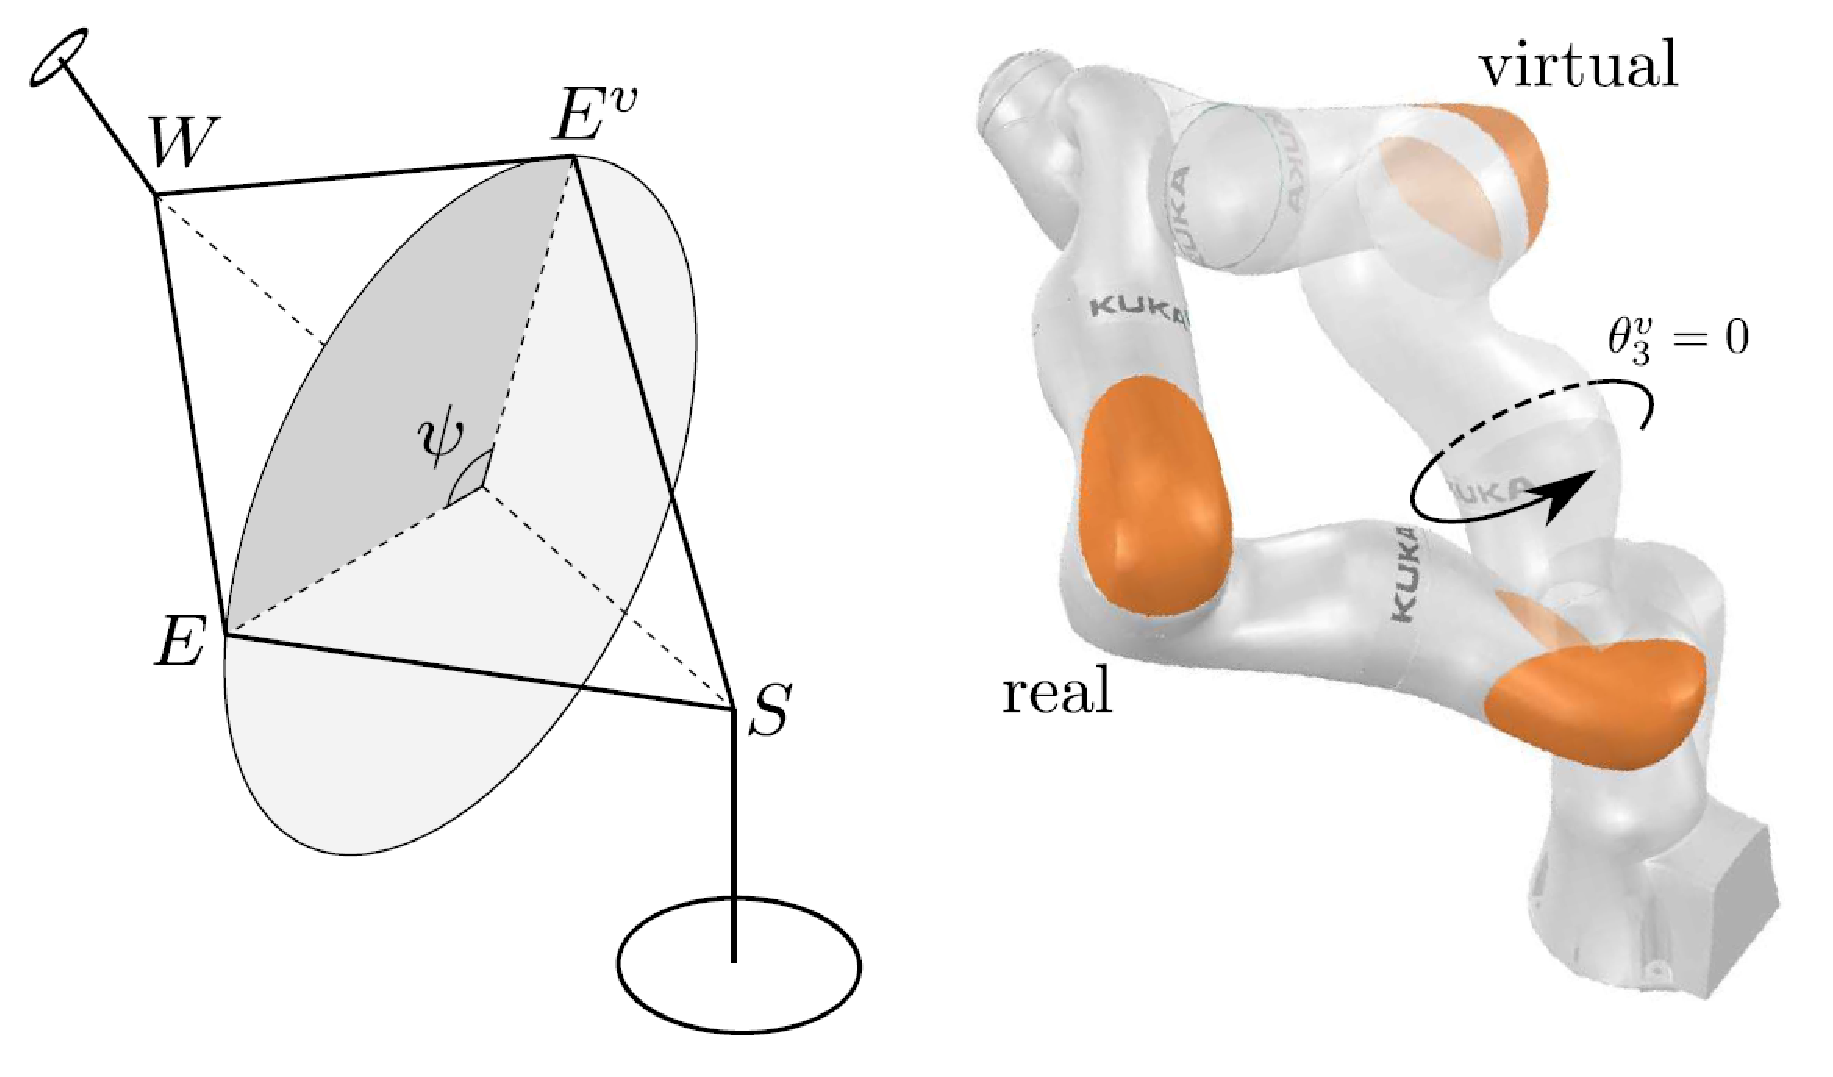
\includegraphics{Elbow_Redudancy.eps}}
	\caption{Der reale Manipulator kann die gewünschte Endeffektor Position in unterschiedlichen Positionen annehmen. Der virtuelle Manipulator wird durch $\theta_3^v=0$ auf sechs Freiheitsgrade reduziert, wodurch für eine globale Konfiguration nur eine Position die gewünschte Endeffektor-Position erreicht. Durch den Unterschied des virtuellen und realen Ellenbogens entsteht ein Winkel $\gamma$ bei der Projektion auf die Schulter-Handgelenks-Geraden.}
	\label{fig:Elbow_redundancy}
\end{figure}

Die Position $x_b^e$ wird durch die homogene Transformation $H_b^e$ vorgegeben, welche die Position $\vec{p}_b^e \in \R^3$ und den Rotationsanteil $R_b^e \in SO(3)$. Die Vektoren zwischen den Gelenken sind durch
\begin{align}
\vec{p}_b^2 &=
\begin{bmatrix}
 0 \, 0 \, d_{bs}
\end{bmatrix}^T
 \\
\vec{p}_2^4 &= 
\begin{bmatrix}
0 \, d_{se} \, 0
\end{bmatrix}^T
\\
\vec{p}_4^6 &=
\begin{bmatrix}
0 \, 0 \, d_{ew}
\end{bmatrix}^T
\\
\vec{p}_6^e &= 
\begin{bmatrix}
0 \, 0 \, d_{wf}
\end{bmatrix}^T
\end{align}
definiert. Zuerst wird der virtuelle Winkel $\theta_4^v$ berechnet, wozu nur die geometrische Struktur und der Schulter-Handgelenk-Vektor benötigt wird. Dieser kann wiederum mit der Position $x_b^e$ durch
\begin{align}
\vec{p}_2^6 = \vec{p}_0^7 - \vec{p}_0^2 - (R_0^7 \, \vec{p}_6^7)
\end{align}
berechnet werden. Damit folgt
\begin{align}
\theta_4^v = GK_4 \arccos \left( \frac{|\vec{p}_2^6|^2-d_{se}^2-d_{ew}^2}{2 d_{se} d_{ew}}\right )
\end{align}
Sofern $\theta_3^v=0$ gilt, liegen der Schulter-Ellenbogen Vektor $\vec{p}_2^4$ sowie der Ellenbogen-Handgelenk Vektor $\vec{p}_4^6$ in der $xy$-Ebene auf einer Geraden, sodass der Winkel $theta_1^v$ dafür verantwortlich ist, wie der Vektor $\vec{p}_2^6$ ausgerichtet ist. Im Fall, dass $\vec{p}_2^6$ in der $z_1$-Achse liegt, würde eine Singularität auftreten, sodass folgende Fallunterscheidung 
\begin{align}
\theta_1^v = 
\begin{cases}
atan2(\vec{p}_2^6)
\end{cases}
\end{align} 
\begin{figure}
	\centering
	\scalebox{0.4}{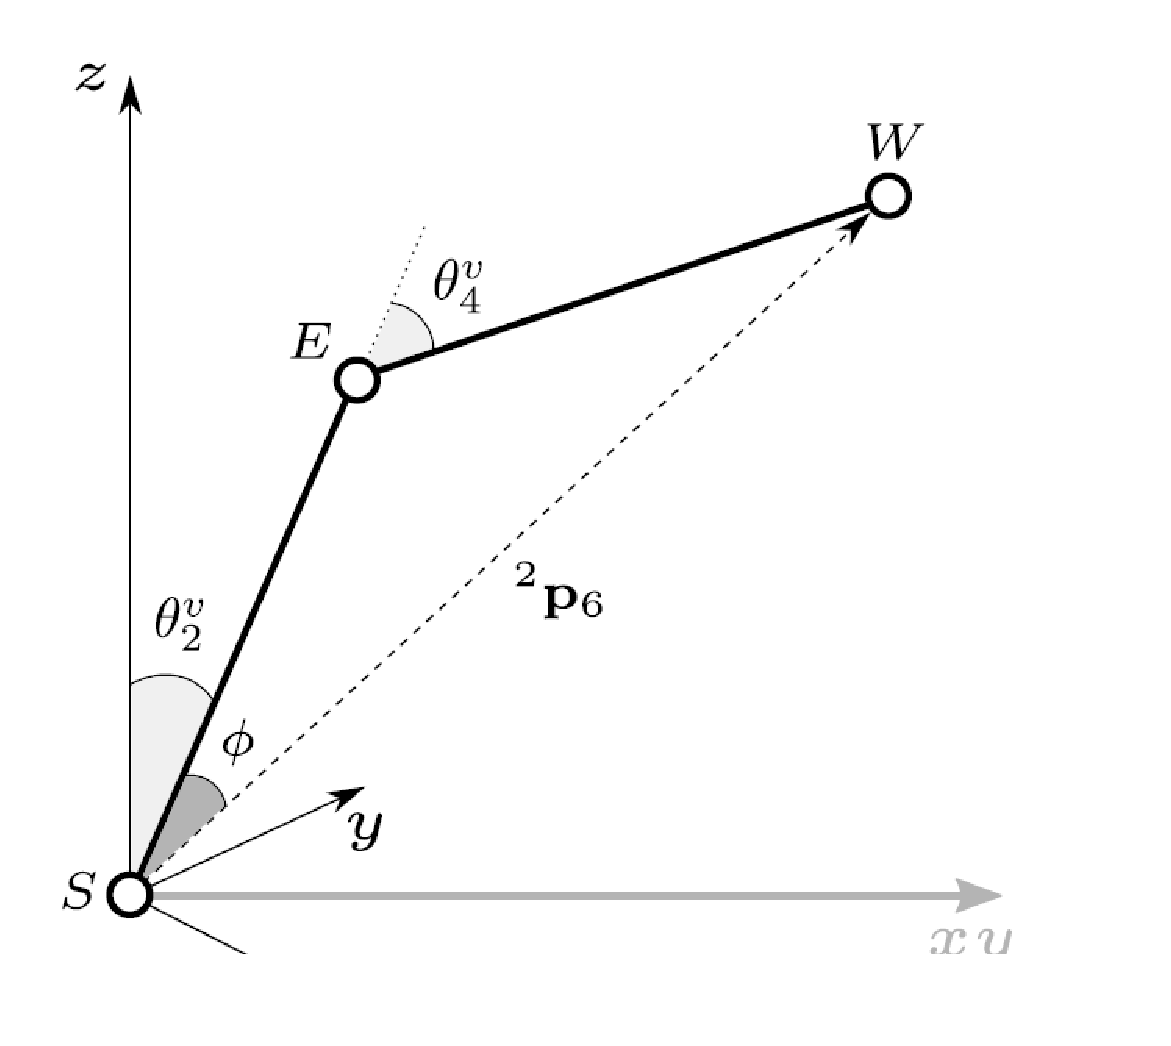
\includegraphics{Theta_4_v_calculation.eps}}
	\caption{Darstellung der Schulter, des Ellenbogens und dem Handgelenk zur Bestimmung von $\theta_4^v$ und $\theta_2^v$.}
	\label{fig:theta_v_calculation}
\end{figure}


%%% Local Variables: 
%%% mode: latex
%%% TeX-master: "main"
%%% End: 
